\newcommand{\objective}[1]{
    \ifnum #1=1
        Introduce \gls*{htm} and give a deep understanding of the inner workings, the strengths, and the weaknesses. While also being easy to grasp for readers with a machine learning background.
    \else \fi
    \ifnum #1=2
        Develop and outline a theoretically sound \gls*{htm} architecture that can be applied for anomaly detection in complex videos.
    \else \fi
    \ifnum #1=3
        Perform experiments, discuss the results, and lay out potential future work for Grid HTM. The experiments will vary in difficulty, complexity, and will focus on different use cases.
    \else \fi
}

\chapter{Introduction}
\label{sec:introduction}
\section{Background and Motivation}
As the global demand for security and automation increases, many seek to use video anomaly detection systems. In the US alone, the surveillance market is expected to reach $\$23.60$ Billion by 2027~\cite{us_video_stats}. Leveraging modern computer vision, modern anomaly detection systems play an important role in increasing monitoring efficiency and reducing the need for expensive live monitoring. Their use cases can vary from detecting faulty products on an assembly line to detecting car accidents on a highway, and everything in between.
\par
The most important component in video anomaly detection systems is the intelligence behind it. The intelligence ranges from simple on-board algorithms to advanced deep learning models, where the latter has experienced increased popularity in the past few years, as can be seen in \autoref{fig:dl_publications}.\par
\begin{figure}[H]
    \centering
    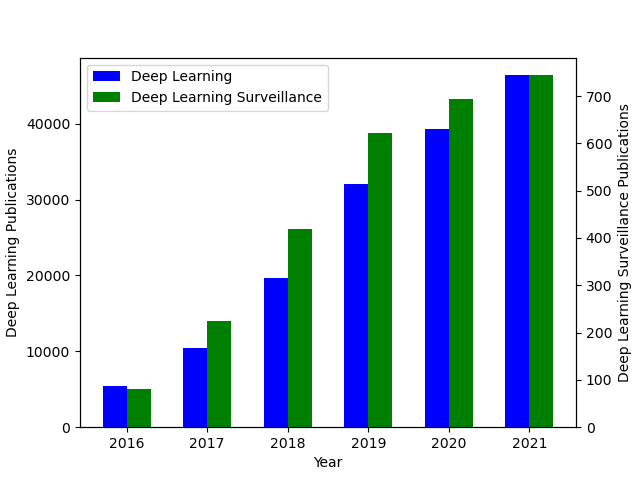
\includegraphics[width=\linewidth]{resources/introduction/publications_graph}
    \caption[Publications Increase Comparison]{The increase in publications mentioning the terms "deep learning" and "deep learning surveillance"~\cite{deep_learning_surveillance_stats}.}
    \label{fig:dl_publications}
\end{figure}
Yet despite the major progress within the field of deep learning, there are still many tasks where humans outperform models, especially in anomaly detection where the anomalies are often undefined. Deep learning approaches also perform poorly when dealing with noise and concept drift.
\par
The cause for the discrepancy lies in the difference between how humans and machine learning algorithms represent data and learn. Most machine learning algorithms use a dense representation of the data and apply back-propagation in order to learn. Human learning happens in the neocortex, where evidence points to that the neocortex uses a sparse representation and performs Hebbian-style learning. For the latter, there is a growing field of machine learning dedicated to replicating the inner mechanics of the neocortex, namely  \gls*{htm} theory. This theory outlines its advantages over standard machine learning, such as noise-tolerance and the ability to adapt to changing data.
\par
With the advantages of  \gls*{htm} and the rise of video anomaly detection in mind, a natural question one could pose is whether it is possible to apply  \gls*{htm} for anomaly detection in videos. Combined with a lack of related works, it is this very question that is the motivation behind this thesis.

\section{Problem Statement}
\label{sec:problem_statement}
Based on the background and motivation, the problem statement can be boiled down to a simple question: \textbf{Is \gls*{htm} viable for use in video anomaly detection?}\par
This thesis will introduce three different objectives that will help answer the question and also showcase the performance of HTM. It will also cover all required knowledge. The objectives are as follows:
\begin{enumerate}
    \item \objective{1}
    \item \objective{2}
    \item \objective{3}
\end{enumerate}

\section{Limitations}
HTM is a complex topic not part of the curriculum in most educations, if any at all. It is also based on neurological research, lending terms and concepts from the biological field, which significantly raises the level of entry for people with a machine learning background. The field also has a low level of accessibility due to a lack of proper documentation and a high reliance on the tiny \gls*{htm} community. This makes learning and understanding \gls*{htm} a process which takes up a sizable chunk out of the total time spent on this thesis. This thesis will therefore be relatively limited in scope.
\par
Additionally, \gls*{htm} for video anomaly detection~\cite{MotionAnomalyDetection} is a novel topic and is therefore naturally limited on several fronts. One of the main limitations is the lack of labeled anomaly data that suits the nature of HTM, because most datasets are made for use with deep learning approaches. Another problem is the lack of works related to applying \gls*{htm} on video-based problems. Finally, while there are other methods that can be used for video anomaly detection, none of them are based on the same premises as HTM. This means that there is a major lack of methods to use for the purpose of benchmarking and comparison.
\par
It should also be mentioned that the \gls*{htm} theory described in this thesis is not the first generation~\cite{htm_zeta1}, which was probabilistic in nature. The \gls*{htm} theory described in this thesis is actually the third generation~\cite{htm_gen3, thousandbrains}, which builds upon the second generation~\cite{htm_gen2_sp,htm_gen2_tm}. The second generation is often referred to as Cortical Learning Algorithms (CLA), which made the move from probabilistic modelling to Sparse Distributed Representation. The third generation builds upon the second generation by introducing concepts such as sensorimotor inference and The Thousand Brains Theory. The first generation had fundamentally different inner workings, but shared a lot of the terms with the current generation. This has made researching  \gls*{htm} challenging as there are many research papers published that refer to the first generation.
\par
Finally, it needs to be noted that Numenta, which is the company behind HTM, is a private for-profit company. This means that it is in their best interest to present \gls*{htm} as a highly functional and powerful machine learning algorithm. This can lead to unhealthy optimism, which has caused complications during the work of this thesis. One should therefore be critical when reading research papers from Numenta, and always keep in mind that they might not only be research papers but may also be marketing materials. It should also be mentioned that this thesis is relying on the community fork~\cite{htm_community_fork} of \gls*{htm} because Numenta has stopped development on the original codebase.

\section{Contributions}
This thesis explores the use of \gls*{htm} for anomaly detection in videos, and introduces a new type of \gls*{htm} architecture called Grid HTM, which requires a vigorous understanding of HTM. The main contributions are therefore achieved through the objectives introduced in \autoref{sec:problem_statement}. How this thesis achieves those objectives is described below:
\paragraph*{Objective 1} \emph{\objective{1}}
\par
This objective is achieved in \autoref{sec:background}, where \gls*{htm} is explained. This chapter also acts as an organization of  \gls*{htm} related research, supported with visualizations and a simpler language, making it easier for people with a machine learning background to understand. It is also important to mention that not only does this chapter include the main \gls*{htm} research published, but it also contains little tidbits of community research and ideas which are otherwise hard to come by.
\paragraph*{Objective 2} \emph{\objective{2}}
\par
This objective is achieved in \autoref{sec:grid_htm}, where Grid \gls*{htm} was introduced. Not only does it present a novel way to apply  \gls*{htm} on video-based problems, it also uncovers the reasoning behind the design decisions that were made as well as providing thorough analysis. This objective is further achieved through the Grid HTM paper, which is a product of this thesis, and can be seen in \autoref{appendix:paper}.
\paragraph*{Objective 3} \emph{\objective{3}}
\par
This objective was achieved in \autoref{sec:experiments}, where three different experiments were performed. The first experiment showcased that \gls*{htm} and Grid \gls*{htm} can indeed perform anomaly detection on simple and clean videos. The second experiment showcased the performance of Grid \gls*{htm} on a complex surveillance video, which showed promising results. The third experiment showcased the ability of Grid \gls*{htm} to detect segments in a video, where noisy videos of sperm were used for increased challenge.
\par
Now that the three objectives have been achieved, it is possible to answer the thesis question: \textbf{Is \gls*{htm} viable for anomaly detection in videos?} The experiments show that with proper data and further refinements, Grid \gls*{htm} and other \gls*{htm} based architectures can indeed be used as anomaly detection systems for videos.
\par
Additionally, during the course of this thesis, a contribution have been made to the  \gls*{htm} community in the form of uncovering and reporting a bug related to the technical implementation of  \gls*{htm}~\cite{github_contrib}. It is also important to reiterate that this thesis acts as a general guide to \gls*{htm} from a machine learning perspective, which is something that is sorely needed due to the low accessibility of the \gls*{htm} field.
\par
Finally, all the work done in this thesis, including the Grid \gls*{htm} source code and the various experiments, is publically available at Github~\cite{master_thesis_github}.
\section{Research Methods}
Due to the novelty of this thesis, a single research method could not be used. Instead, a combination of multiple research methods was employed. For most of the thesis, an exploratory research method was used with the context of answering the thesis question, this was used due to the novelty of this thesis and the lack of related works. The result of this exploratory method is Grid HTM, which began from a simple starting point and was shaped through exploring improvements and solutions to problems that arose.
\par
For the surveillance experiment, a qualitative research method was used to determine the effectiveness of Grid HTM. This is due to the lack of labeled data which made it hard to quantify, and that real life surveillance examples are complex by nature. The result is that the effectiveness was determined not through numbers, but through whether the results were qualitatively reasonable.
\par
As for the other experiments, a more quantitative research method was used. This was made possible in the bouncing ball experiment due to the controlled nature of the experiment. In the sperm experiment, this was made possible due to the use of a benchmark, which allowed for direct comparisons.
\section{Thesis Outline}
This thesis consists of five chapters, where \autoref{sec:introduction} and \autoref{sec:background} are introductory and contain relevant background information for the understanding of the proceeding chapters. \autoref{sec:grid_htm} and \autoref{sec:experiments} present the work done during this thesis. \autoref{sec:conclusion} neatly summarizes this thesis and presents areas in which there can be performed further work. More details for each of the chapters, except this one, is presented below.
\par
\subsection*{Chapter 2: Background}
\autoref{sec:background} covers the required knowledge for the proceeding chapters, as well as a short section about ethical considerations. It is split up into three parts. The first part covers deep learning and its history, and has an increased focus on the parts of deep learning that are especially relevant for this thesis, such as generative models.
\par
The second part covers anomaly detection. More specifically, it covers the definition, challenges, and recent work within anomaly detection. It also discusses smart surveillance, which is a subset of anomaly detection specifically meant for surveillance purposes.
\par
The third and final part covers \gls*{htm} theory. It starts off by introducing the biological ties to \gls*{htm} and the pipeline of an \gls*{htm} model. This is then proceeded by a detailed account of the inner mechanisms of an \gls*{htm} model and how learning is performed. It then finishes by introducing use-cases, related work on the use of \gls*{htm} for anomaly detection and how it performs, and introduces similarities between recent developments within \gls*{htm} theory and recent developments within deep learning.
\subsection*{Chapter 3: Grid HTM}
This chapter introduces Grid HTM, a novel \gls*{htm} architecture for the purpose of anomaly detection in videos, which is the main contribution of this thesis.
\par
Grid \gls*{htm} is presented gradually as problems occur and have to be solved. Some of these problems are invariance and unstable anomaly output. The technicalities are explained with the help of figures and various analyses. This architecture is then used in \autoref{sec:experiments} when performing experiments.
\par
Potential use cases are presented, such as reducing the need for expensive live monitoring as well as anomaly data labeling. The biological plausibility is also briefly discussed, and concludes that Grid \gls*{htm} may loosely be considered a cortical region.
\subsection*{Chapter 4: Experiments and Results}
This chapter presents three experiments that aim to explore the capabilities and challenges of \gls*{htm} and Grid \gls*{htm} in the context of anomaly detection in videos. The first experiment is a controlled experiment where a computer-generated ball is bouncing with anomalies inserted. The aim of this experiment is to test whether the capabilities of \gls*{htm} apply for videos, as well as the performance of Grid \gls*{htm} on the same task.
\par
The second experiment showcases the performance of Grid \gls*{htm} on a surveillance video with technical anomalies. Additionally, several key points of interests and the respective outputs of Grid \gls*{htm} are shown in order to get a better understanding of its capabilities.
\par
The third experiment further explores the ability of the Grid \gls*{htm} to detect segments in videos, which was discovered in the previous experiment. The videos that are used in this experiment are videos of sperm that contain several segments.
\subsection*{Chapter 5: Conclusion and Further Work}
In this chapter the thesis is summarized, and the thesis question presented in \autoref{sec:introduction} is answered along with potential further work and the main contributions of this thesis.
\par
The contributions are presented as the description of how the various objectives were achieved, as well as answering the thesis question. This is a shorter version of the contributions mentioned in the introduction, and is presented conclusively.
\par
This chapter also presents potential future work, which is further divided into sections focusing on different aspects such as datasets, Grid HTM, HTM and deep learning, and general research progress.